\section{Flag 11 - Survey}

\paragraph{03A944B434D5BAFF05F46C4BEDE5792551A2595574BCAFC9A6E25F67C382CCAA}
\begin{center}
    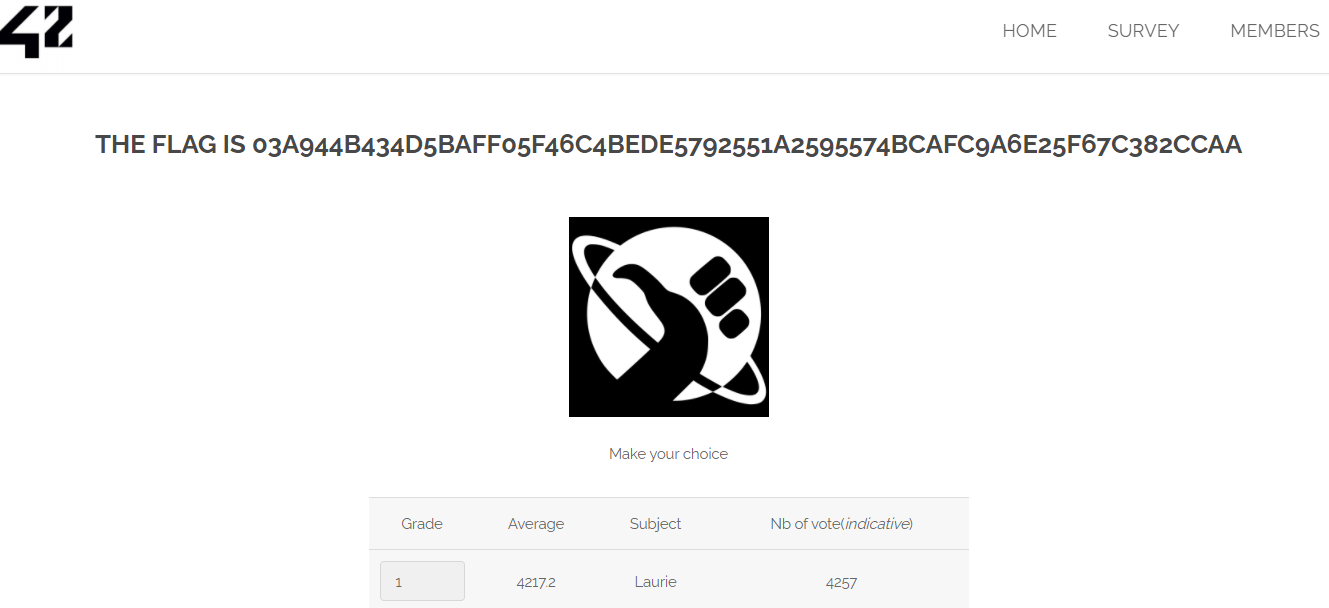
\includegraphics[width=0.5\textwidth]{14.Flag11/11-05.png}\\[0cm] 
\end{center}

\subsection{Vulnerability}

The html components listed in the survey are editable and are parsed from the front end. Idealy these values should be stored in the back and the value kept in the front should determine where in the array they are kept

Or simply, keep the form as "READ ONLY"

This will easily tamper with collected input or data sent to database.

\subsection{Location}

`http://<ip-address>:80/index.php?page=survey`

\subsection{Method}

On the survey page, open the Inspection Tool and select the drop-down boxes. You will see the code looks something like:

```

<tr bgcolor="Silver">

    <td align="center">
    
        <form action="\#" method="post">
    
        <input type="hidden" name="sujet" value="2">
    
        <SELECT name="valeur" onChange='javascript:this.form.submit();'>
    
            <option value="1">1</option>
      
            <option value="2">2</option>
      
            <option value="3">3</option>
      
            <option value="4">4</option>
      
            <option value="5">5</option>
      
            <option value="6">6</option>
      
            <option value="7">7</option>
      
            <option value="8">8</option>
      
            <option value="9">9</option>
      
            <option value="10">10</option>
        
        </SELECT>
  
    </form>

</td>

```

I changed one of the values to match a telephone number, like this:

```

<option value="27124274000">10</option>

```

the flag was then return after selecting that value.


\subsection{Tools}

\begin{figure}[!htb]
    \centering
    \subfloat[Where]{
\includegraphics[width=.45\columnwidth]{14.Flag11/11-01.png}\label{fig: 11-01 - wtf}} \quad
    \subfloat[Survey]{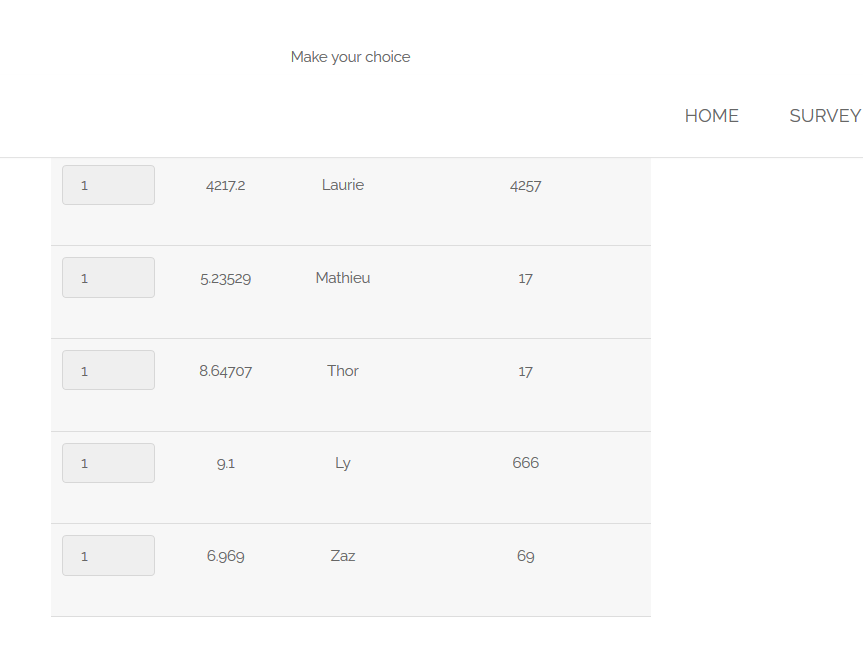
\includegraphics[width=.45\columnwidth]{14.Flag11/11-02.png}\label{fig: 11-02 - wrong}} \\
    \subfloat[Inspect an Option]{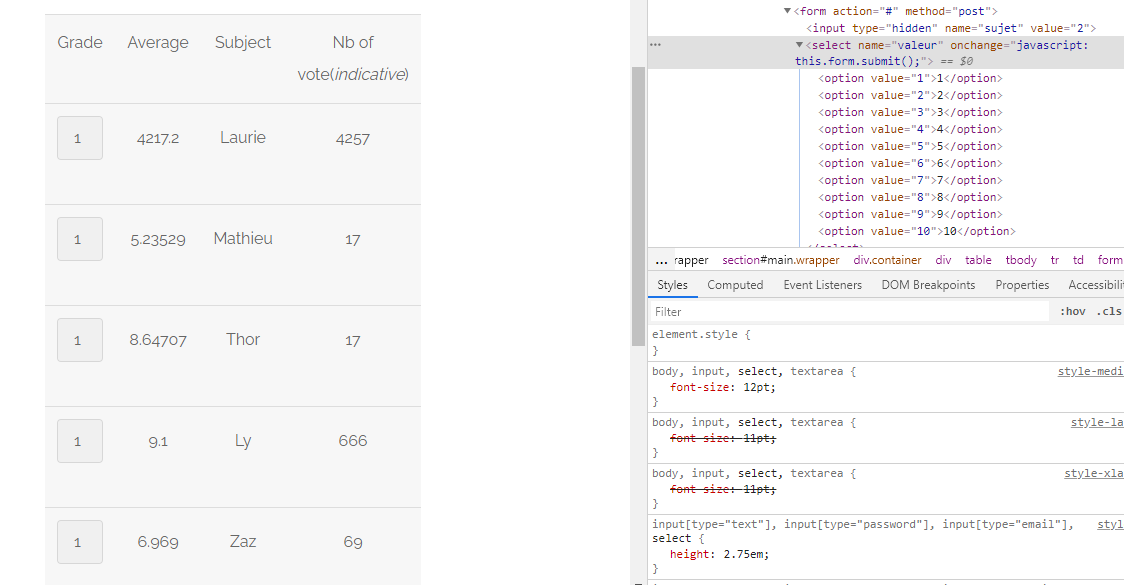
\includegraphics[width=.45\columnwidth]{14.Flag11/11-03.png}\label{fig: 11-03 - wtf}} \quad
    \subfloat[Change to Telephone number]{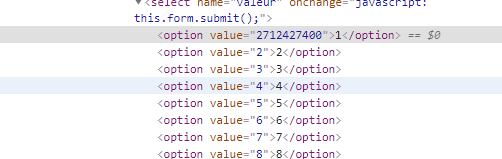
\includegraphics[width=.45\columnwidth]{14.Flag11/11-04.png}\label{fig: 11-04 - wrong}} \\
    \caption[Flag 11 Method]{Process to Capture the Survey Flag} % The text in the square bracket is the caption for the list of figures while the text in the curly brackets is the figure caption
    \label{fig:flag11 method}
\end{figure}

\begin{itemize}
    \item Google Chrome Inspection Tool
    \item \href{https://owasp.org/www-community/attacks/Web\_Parameter\_Tampering}{OWASP}
\end{itemize}

\subsection{Remedy}

\begin{itemize}
    \item Make the form read-only
    \item Verify and Sanitise input
    \item Rather store information for input in the backend than accept raw html input.
\end{itemize}
